\documentclass[11pt]{beamer}
\usetheme{Warsaw}
\usefonttheme{serif}

\newcommand*\oldmacro{}%
\let\oldmacro\insertshorttitle%
\renewcommand*\insertshorttitle{%
  \oldmacro\hfill%
  \insertframenumber\,/\,\inserttotalframenumber}

\let\olditem=\item% 
\renewcommand{\item}{\olditem \justifying}%


\usepackage{makecell}
\usepackage[utf8]{inputenc}
\usepackage[T1]{fontenc}
\usepackage[french]{babel}
%\usepackage[english]{babel}
\usepackage{ragged2e}
\usepackage{graphicx}
\usepackage{caption}
\usepackage{subcaption}
\usepackage{xcolor}
\usepackage{tcolorbox}
\usepackage{float}
\usepackage{booktabs}
\usepackage{multirow}
\usepackage{array}
\usepackage{tabularx}
\usepackage{graphicx}
\usepackage{longtable}
\justifying
% Setup
\graphicspath{{img/}}
\logo{
\includegraphics[height=5mm]{img/logouniv.png}}

% Metadata
\title{Représentation des connaissances spatiales et modélisation de l'apprentissage des agents pour la simulation de l'utilisation de la terre}
\subtitle{}

%%%%%%%%%%%%%%%%%%%%%%%%%%%%%%%%%%%%%%%%%%%%%%%%%%%%%%%%%%%%%%%%%%%%
\begin{document}
 \begin{frame}[plain]
    % Header
    \begin{figure}
      \vspace{-0.5cm}
      \centering      
      
\includegraphics[width=.8\textwidth]{univ-header.png}
    \end{figure}
    \vspace{-1.2cm}

    % Title
    \author{}
    \date{}
    \titlepage
    \vspace{-2.5cm}
    
    % Authoring
    \centering
    {
      \scriptsize
      
      Par\\[1mm]
      {\bfseries NGOMSEM Ngueramadji}\\[1mm]
      CM-UDS-23SCI0912\\[3mm]
      
      Sous la direction de\\[1mm]
      {\bfseries Dr FOTSING Eric}\\[1mm]
      {\itshape Chargé de cours, Université de Dschang/IUT}\\[3mm]
      
      {\normalsize {\today}} 
    }    
  \end{frame}
\author{NGOMSEM Ngueramadji}
  \begin{frame}
\frametitle{Plan de présentation}
\tableofcontents[hideallsubsections]
\end{frame}
  
  \section{Introduction}
  \subsection{Contexte}
  \begin{frame}
  \frametitle{Contexte}
  La chasse dans les écosystèmes implique des interactions complexes entre prédateurs, proies et ressources.
Les modèles actuels manquent de représentations sémantiques et de généralisation pour capturer ces dynamiques.

\end{frame}
\subsection{Problématique}
\begin{frame}
    \frametitle{Problématique}
    \begin{block}{Problématique}
        Comment modéliser un système multi-agent combinant une ontologie et l'apprentissage pour simuler la chasse de manière réaliste ?
        \end{block}
        \begin{figure}
            \centering
            
\includegraphics[width=0.25\linewidth]{question-1015308_1280.jpg}
            % \caption{Enter Caption}
            \label{fig:enter-label}
        \end{figure}
\end{frame}
\subsection{Objectif général}
\begin{frame}
\frametitle{Objectif général}
\begin{block}{Objectif général}
  L’ambition majeure de cette recherche est la conception et
l’implémentation d’un modèle multi agent, basé sur la
simulation de la chasse.  
\end{block}
   \begin{figure}
        \centering
        
\includegraphics[width=0.25\linewidth]{images.jpeg}
        % \caption{Enter Caption}
        \label{fig:enter-label}
    \end{figure} 
\end{frame}
\subsubsection{Objectifs spécifiques}
\begin{frame}
\frametitle{Objectifs spécifiques}

        \begin{block}{Objectifs spécifiques}
         \begin{itemize}   
        
        \item Modéliser les entités de la chasse sous forme d’agents autonomes ;
        \item Concevoir une ontologie de la chasse pour structurer les connaissances utiles à la
             prise de décision ;
        \item Implémenter des mécanismes d’apprentissage pour permettre aux agents d’adapter leur stratégie ;
    \end{itemize}
    \end{block}
\end{frame}

\subsection{Motivation}
\begin{frame}

\frametitle{Motivation}
    \begin{block}{Pourquoi ce travail ?}
        \begin{itemize}
            \item Lacunes des approches actuelles : absence de sémantique, complexité computationnelle, manque de généralisation.

            \item Scientifique : Explorer l’intégration de l’ontologie et du Q-learning pour modéliser des comportements adaptatifs dans des écosystèmes complexes.

            \item Écologique : Évaluer l’impact de la chasse et des ressources spatiales sur la durabilité des écosystèmes.

            \item Pratique : Proposer un modèle accessible sur GAMA, réutilisable pour la gestion environnementale.

            
        \end{itemize}
    \end{block}
    
\end{frame}
\subsection{Définitions des concepts clés}
\begin{frame}
\frametitle{Définitions des concepts clés}
    \begin{block}{Concepts fondamentaux}
        \begin{itemize}
            \item \textbf{Ontologie} : Structure sémantique définissant les entités (ex. : point d’eau, proie) et leurs relations.
            \item \textbf{Q-learning} : Algorithme d’apprentissage par renforcement sans modèle, basé sur la maximisation de récompenses.
            % \item \textbf{GAMA} : Plateforme de simulation multi-agent pour modéliser des interactions spatiales et temporelles.
            \item \textbf{Dynamiques écologiques} : Évolution des interactions agents-ressources dans le temps.
        \end{itemize}
    \end{block}
\end{frame}
\begin{frame}
\frametitle{Représentation d'un agent et Q_learning}
\begin{figure}
        \centering
        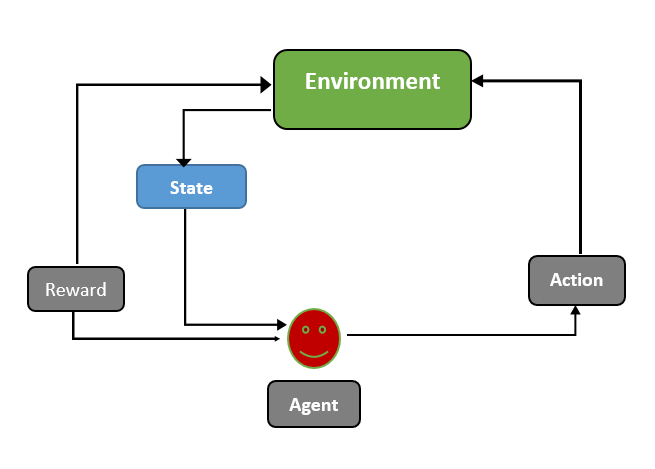
\includegraphics[width=0.9\linewidth, , height=0.8\textheight]{Mes_images/Agent (1).png}
    \end{figure}  
    
\end{frame}
\section{État de l'art}
\subsection{Quelques travaux récents effectués}
\begin{frame}
    \frametitle{Quelques travaux récents effectués}
    \begin{itemize}
\item \textbf{Predicting Ecosystem Resilience (Strannegård et al.):} Utilise le MARL (Multi-Agent Reinforcement Learning) pour modéliser les interactions proie-prédateur dans un environnement alpin\\
Données réelles intégrées, mais  absence d’ontologie, limitant la structuration sémantique de l’espace.

\item \textbf{Collaborative Hunting (Tsutsui et al.):} Repose sur le Deep RL pour simuler la chasse en groupe entre agents.
Modèle collaboratif, mais  ne prend pas en compte les ressources spatiales (eau, herbe), ce qui limite le réalisme écologique.
\end{itemize}
\end{frame}
\begin{frame}
\frametitle{Quelques travaux récents effectués}
 \begin{itemize}
\item \textbf{Agent-Based Modeling (Iwamura et al.):}
Utilise des règles statiques dans un modèle multi-agent classique, avec données empiriques.
Faible capacité d’adaptation des agents ; pas d’apprentissage.
Valide expérimentalement des dynamiques territoriales.
\item   \textbf{Survey on RL(Di Zhang et al.) (2024):}
 Étude théorique des approches d’apprentissage par renforcement.
 Elle ne propose pas de modèle concret, ni d’application à un cas particulier comme la chasse.

 \end{itemize}   
\end{frame}

\subsection{Lacunes identifiées dans les travaux existants}
\begin{frame}
\frametitle{ Lacunes identifiées dans les travaux existants}
\begin{block}{Lacunes identifiés et positionnement de notre approche}
\begin{itemize}
    \item Absence de structuration sémantique des connaissances;
    \item Complexité computationnelle excessive;
    \item Manque d’apprentissage adaptatif;
    \item Manque d’intégration des ressources 
\end{itemize}
\end{block}
\begin{block}{Approche proposée}
    \begin{itemize}
        \item Ontologie pour la représentation sémantique
        \item Q-learning pour l’efficacité
        \item Généralisation 
        \item Approche hybride(ontologie, apprentissage).
    \end{itemize}
\end{block}
    
\end{frame}
\section{Contribution}
    \subsection{Architecture du système}
    \begin{frame}
    \frametitle{Architecture générale du système}
      \begin{figure}
        \centering
        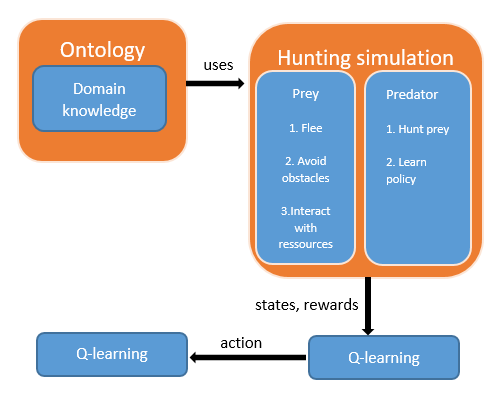
\includegraphics[width=0.9\linewidth, , height=0.8\textheight]{Mes_images/Architecture.PNG}
    \end{figure}  
    \end{frame}
\section{ Expérimentation}
\subsubsection{Outils utilisés}
\begin{frame}
\frametitle{Outils utilisés et langages}
\begin{block}{Outils}
\begin{itemize}
    \item GIS Agent Based Modeling Architecture, plateforme de modélisation multi-agent intégrant JAVA et OWL2;
    \item PC HP Elitebook pro avec les caratéristiques: 
    % \begin{itemize}
    \begin{itemize}
         \item 1T SSD;
         \item 16RAM;
         \item Corei7.    
        \end{itemize}
    % \end{itemize}
    % \item Protrégé.
\end{itemize} 

\end{block}    
\end{frame}
% \subsection{Interface de simulation}
\subsubsection{Ontologie construite}
    \begin{frame}
    \frametitle{Ontologie construite}
    \begin{figure}
        \centering
    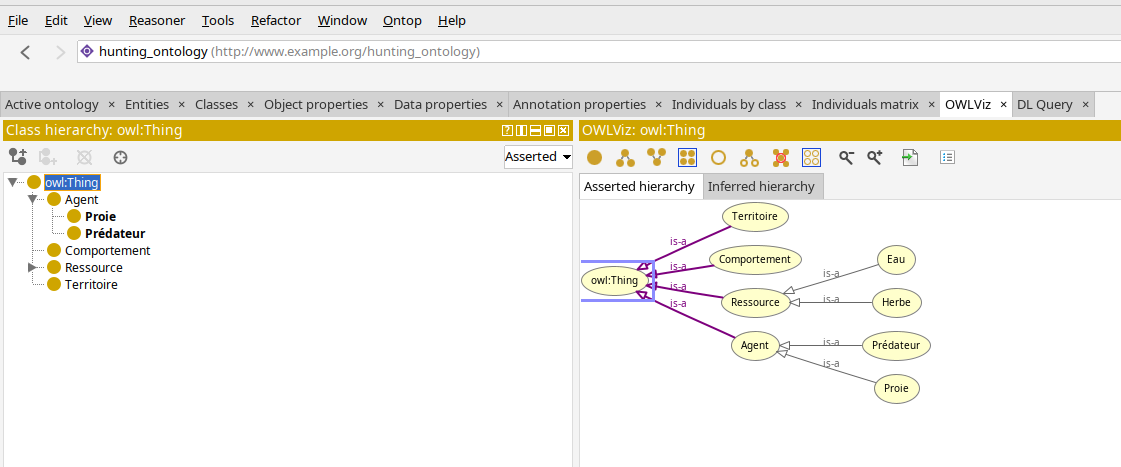
\includegraphics[width=1.2\linewidth, , height=0.9\textheight]{Mes_images/Ontologie créée sous protégé.png}
    \end{figure} 
        
    \end{frame}
\subsubsection{Interface de la simulation}
\begin{frame}
\frametitle{Interface de la simulation}
 \begin{figure}
        \centering
        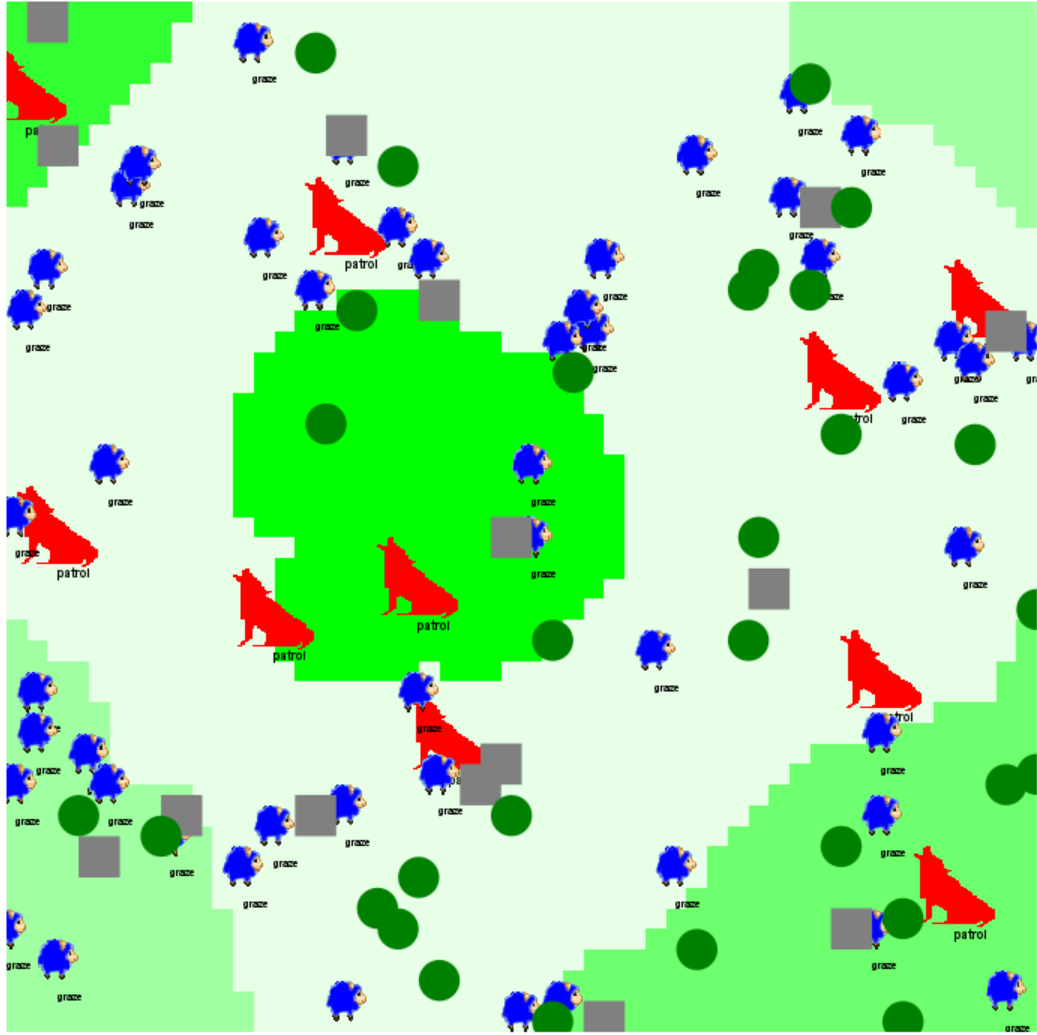
\includegraphics[width=0.9\linewidth, , height=0.8\textheight]{mes_resultats/Interface de simulation.png}
    \end{figure}   
\end{frame}
\subsection{Résultats}
\subsubsection{Évolution des populations}
\begin{frame}
\frametitle{Évolution des populations}
   \begin{figure}
        \centering
        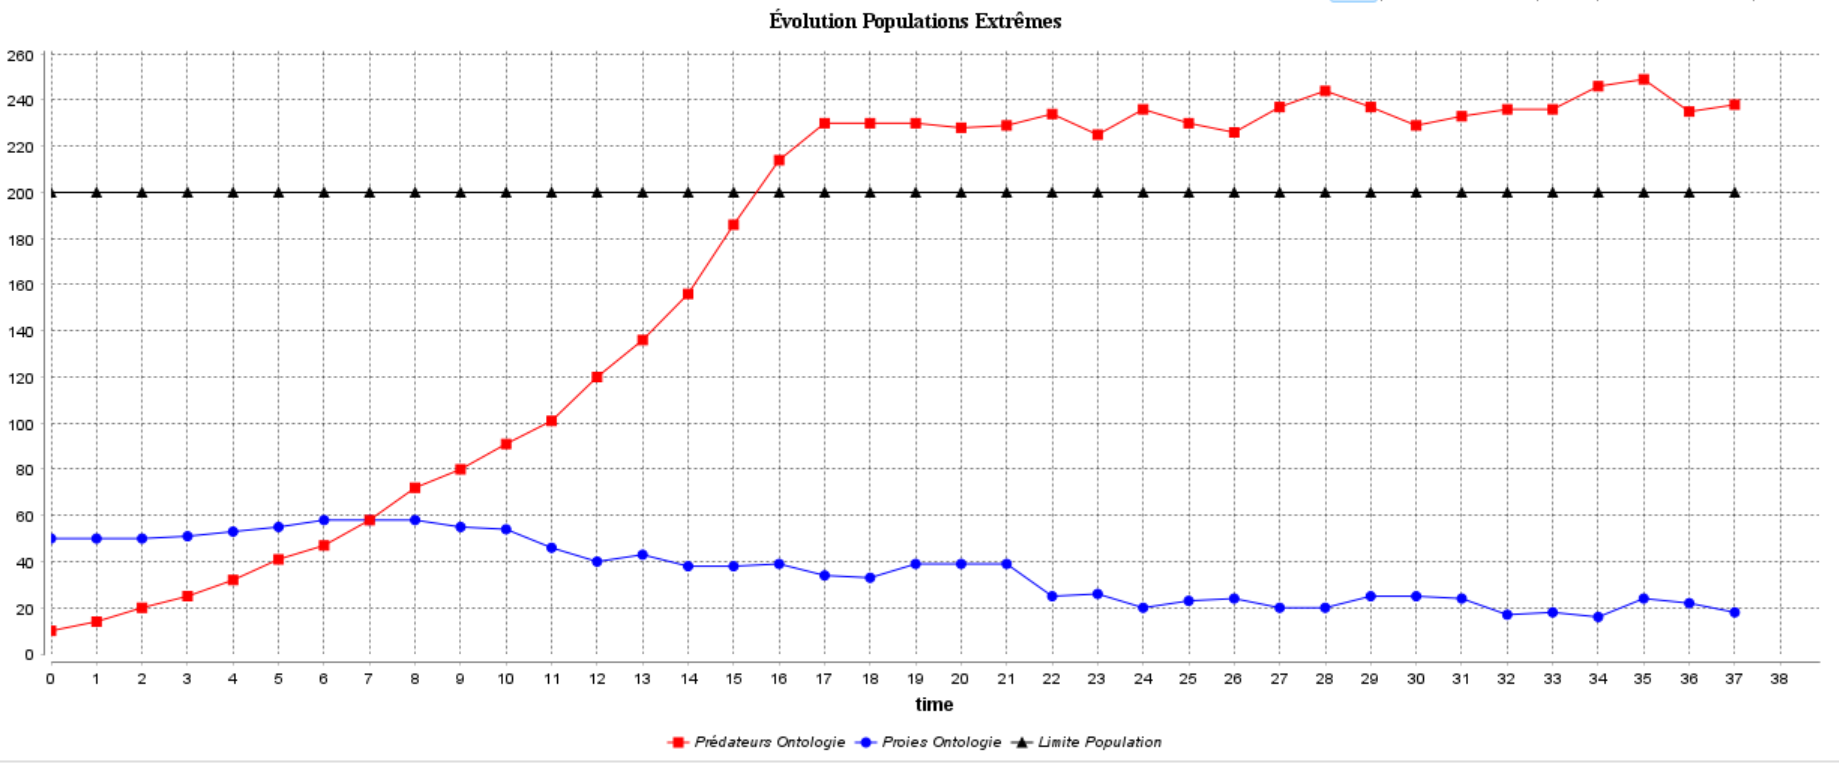
\includegraphics[width=0.9\linewidth, , height=0.8\textheight]{mes_resultats/Evolution des populations.png}
    \end{figure}    
\end{frame}
\subsubsection{Energie moyenne par type}
\begin{frame}
\frametitle{Energie moyenne par type}
   \begin{figure}
        \centering
        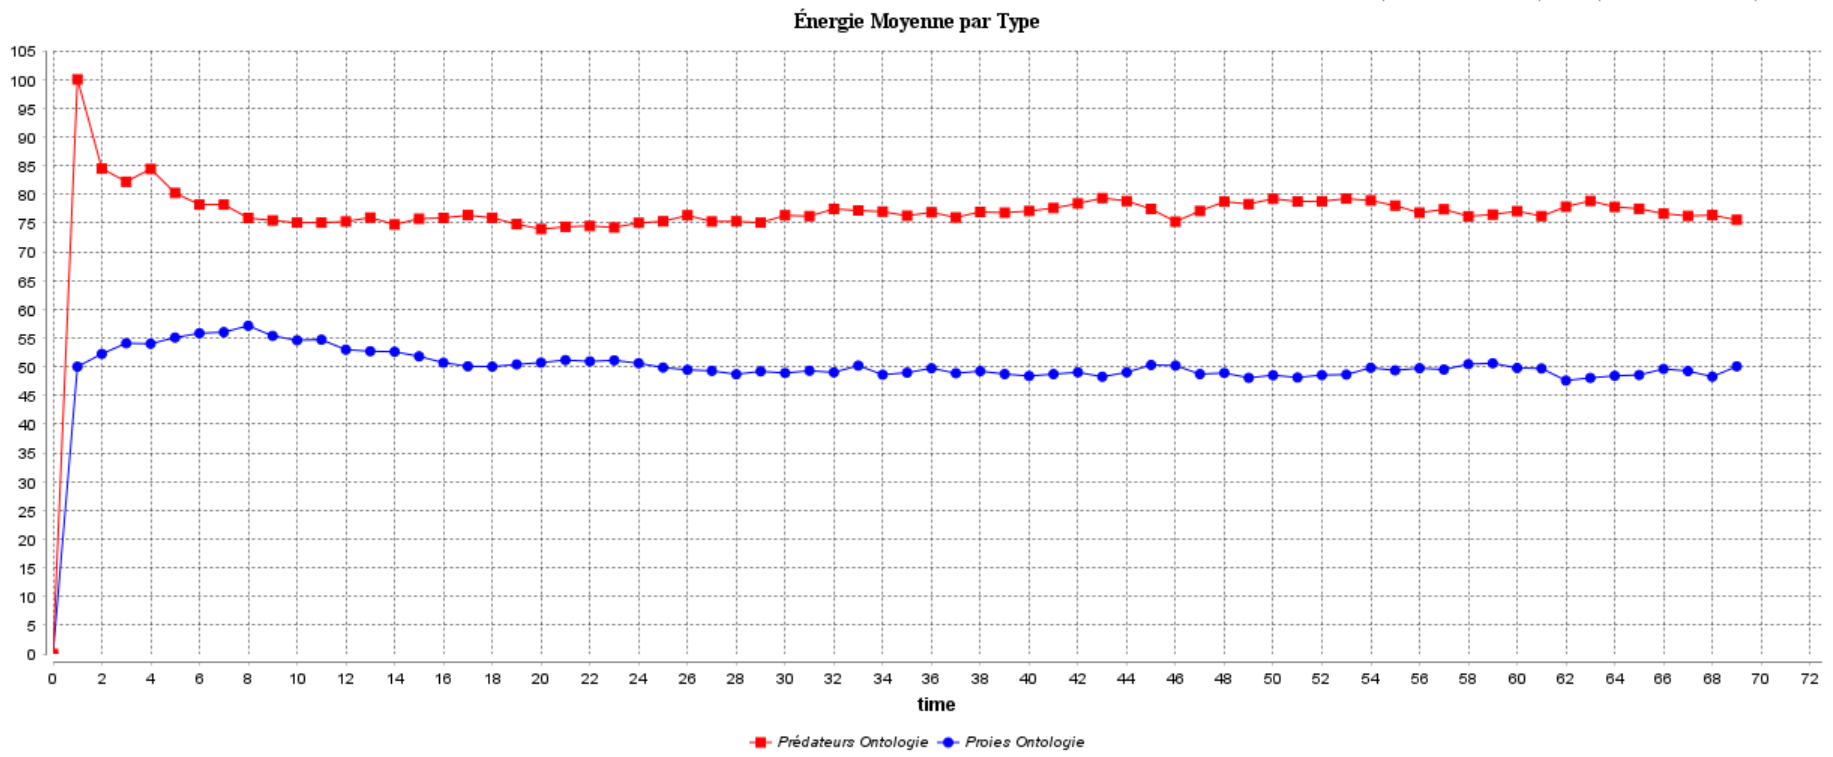
\includegraphics[width=0.9\linewidth, , height=0.8\textheight]{mes_resultats/Energie moyenne par type.png}
    \end{figure}    
\end{frame}
\subsubsection{Naissances cumulées}
\begin{frame}
\frametitle{Naissances cumulées}
   \begin{figure}
        \centering
        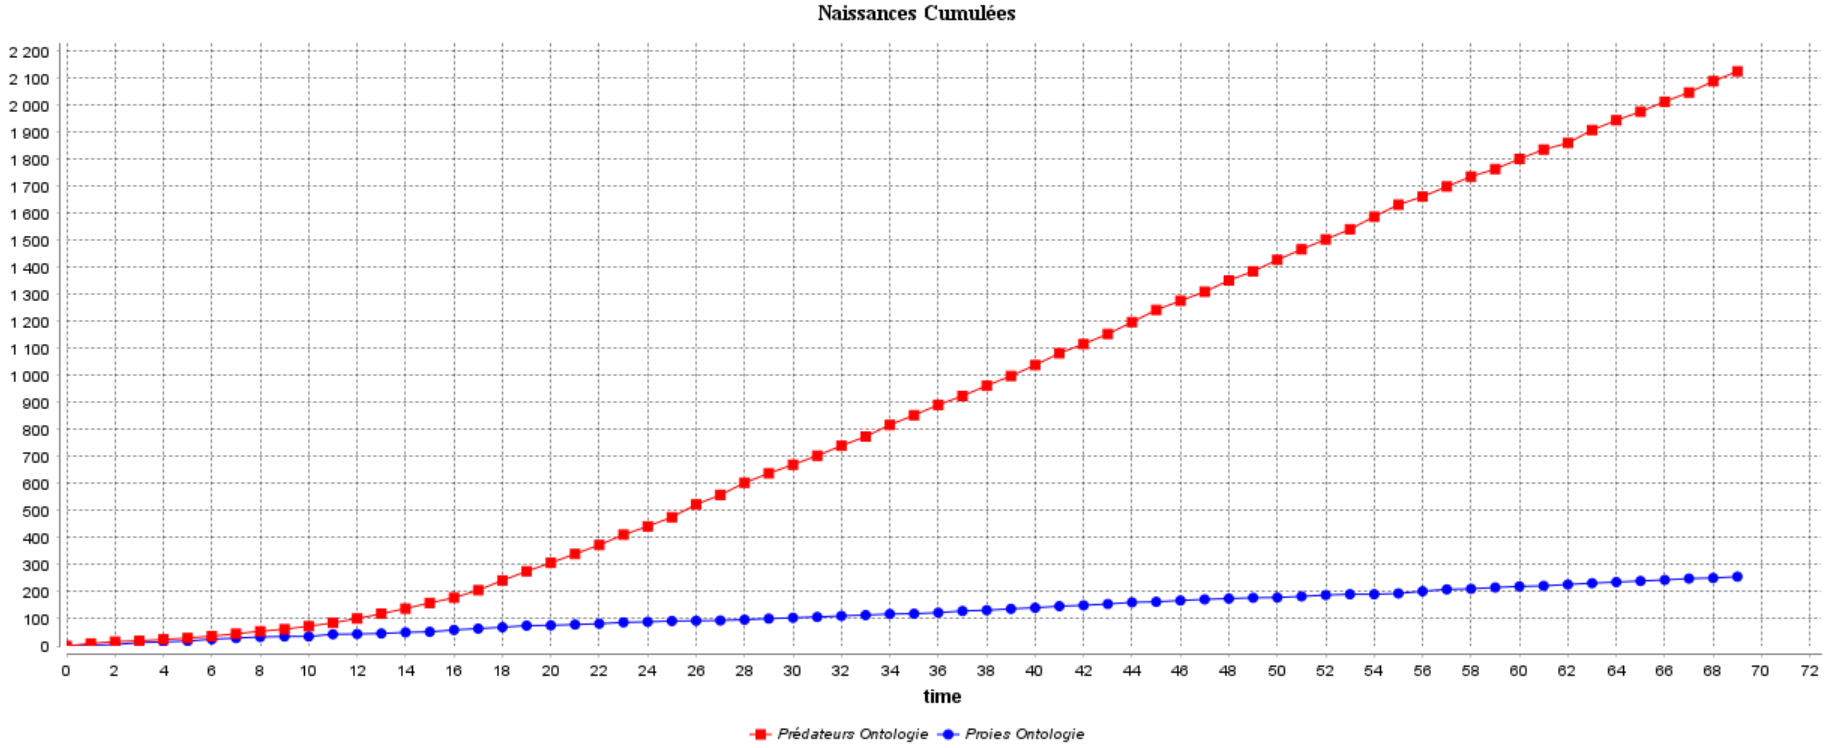
\includegraphics[width=0.9\linewidth, , height=0.8\textheight]{mes_resultats/Naissances cumulées.png}
    \end{figure} 

\end{frame}
\subsubsection{Taux de succès}
\begin{frame}
\frametitle{Taux de succès}
   \begin{figure}
        \centering
        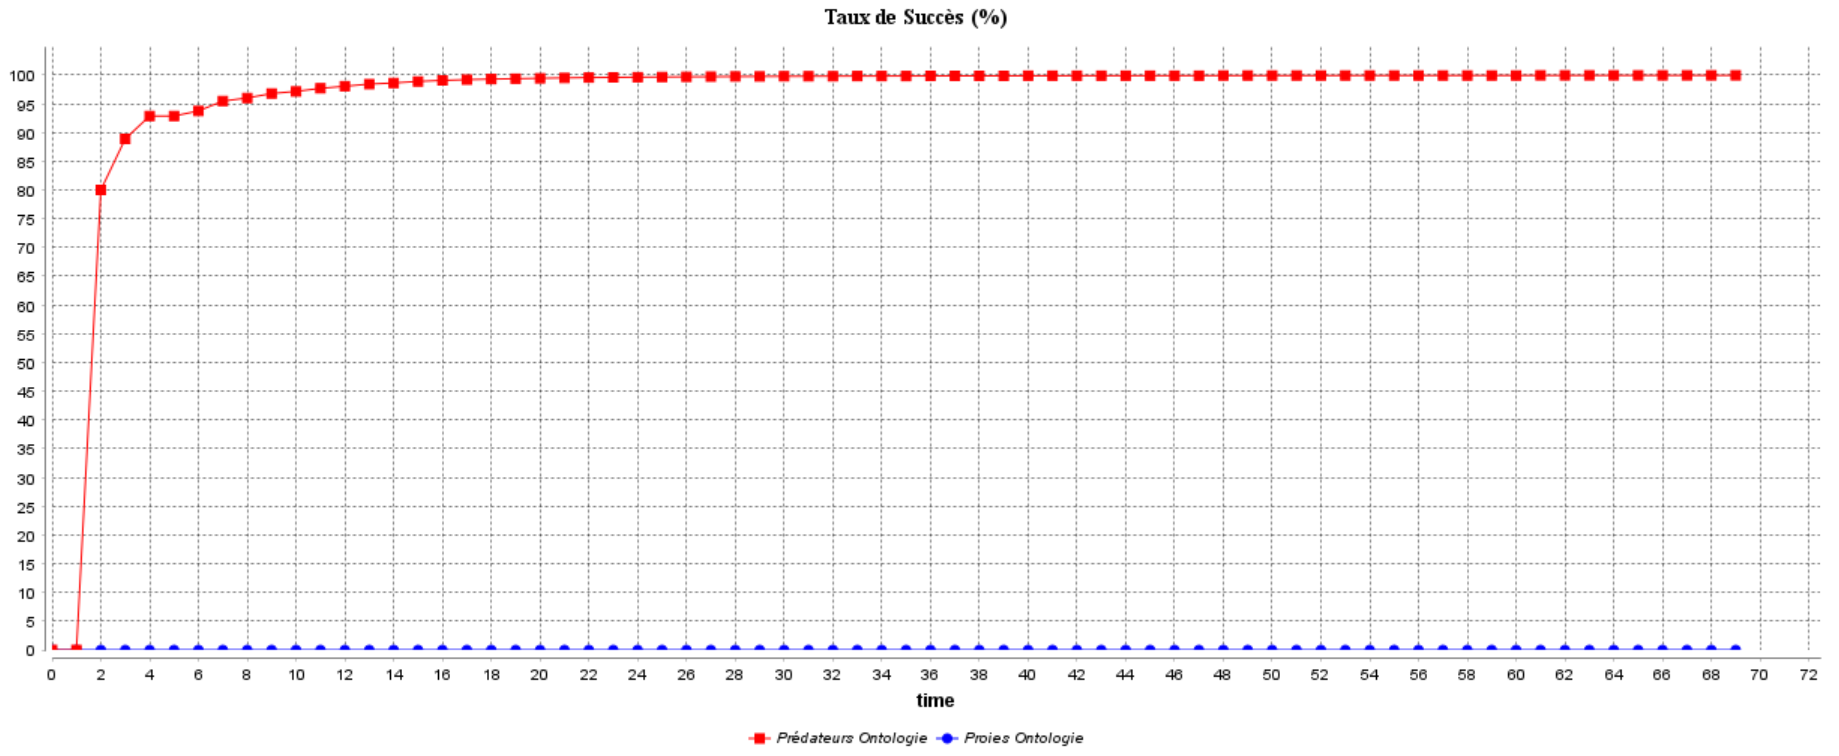
\includegraphics[width=0.9\linewidth, , height=0.8\textheight]{mes_resultats/Taux de succès.png}
    \end{figure}    
\end{frame}
\subsection{Discussion}
% \subsection{Discussion}
\begin{frame}{Comparaison avec les approches de l’état de l’art}
    \begin{table}[H]
        \centering
        \caption{Comparaison basée sur Ontologie, Learning et Génération}
        \begin{tabular}{|p{4.5cm}|p{1.70cm}|p{1.70cm}|p{2cm}|}
            \hline
            \textbf{Approach/Tools} & \textbf{Ontologie} & \textbf{Learning} & \textbf{Génération} \\ \hline
            Notre approche & Y & Auto & Auto \\ \hline
            Collaborative Hunting (Tsutsui et al.) & N & Man & Auto \\ \hline
            Predicting Ecosystem Resilience (Strannegård et al.) & N & Auto & Auto \\ \hline
            Survey on RL(Di Zhang et al.) & N & Man & Man \\ \hline
            Agent-Based Modeling (Iwamura et al.) & N & Man & Auto \\ \hline
        \end{tabular}
        \begin{flushleft}
            % \scriptsize Ontologie: Y=Yes, N=No; Learning: Auto=Automatic, Man=Manual; Génération: Auto=Automatic, Man=Manual
        \end{flushleft}
    \end{table}
\end{frame}
    
\section{ Conclusion}
\subsection{Bilan}
\begin{frame}
\frametitle{ Bilan}
\begin{itemize}
    \item Ce mémoire a permis de concevoir un modèle multi-agent intelligent pour simuler la chasse, combinant ontologie et Q-learning dans GAMA.
    \item Les résultats valident la capacité des agents à apprendre, à interagir de façon crédible avec l’environnement et à optimiser l’usage de l’espace.
    \item L’intégration sémantique améliore la stabilité des dynamiques émergentes par rapport aux approches classiques.
    \item Des limites subsistent, notamment l’absence de données empiriques et la complexité de l’ontologie en environnement dynamique nous ouvrent la porte pour les perspectives futures. 
\end{itemize}
\end{frame}

 
\subsection{Perspectives}
\begin{frame}
\frametitle{Perspectives}
 \begin{itemize}
    \item Intégration de données empiriques pour une validation plus robuste.
    \item Extension du modèle à d’autres écosystèmes (ex. : zones humides, déserts).
     \item Optimisation des algorithmes pour des simulations à plus grande échelle.
    % \item Collaboration avec des écologistes pour des applications pratiques.


 \end{itemize}   
\end{frame}

\begin{frame}
\begin{figure}
        \centering
        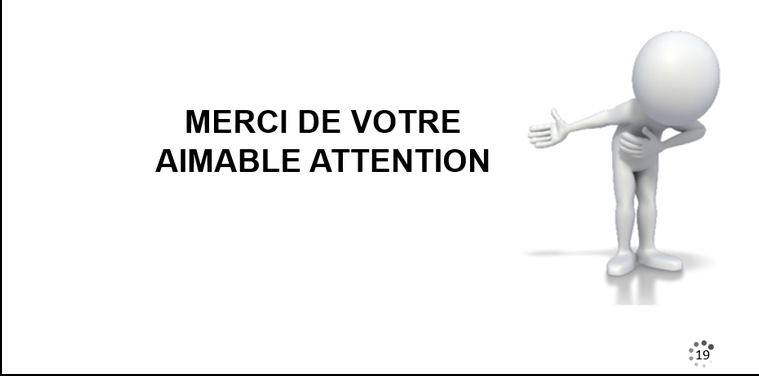
\includegraphics[width=0.9\linewidth, , height=0.8\textheight]{Capture d’écran du 2025-07-21 00-54-31.png}
\end{figure} 
    
\end{frame}
\end{document}
\end{document}